\documentclass[a4paper,11pt]{article}

\usepackage[utf8]{inputenc}
\usepackage{mathpazo}
\usepackage{gensymb}
\usepackage{graphicx}
\usepackage{url}
\usepackage[frenchb]{babel}
\usepackage{subfig}
\usepackage{apacite}
\usepackage{array}
\usepackage{multirow}
\usepackage{dcolumn}
\newcolumntype{d}[1]{D{,}{,}{#1}}
\usepackage[T1]{fontenc}
\usepackage{amsmath}

\begin{document}

\title{Fastqc \& Multiqc review}
\author{Marilyne Aza-Gnandji}
\date{\today}

\maketitle
\tableofcontents

\section{Généralités}

FastQC est un logiciel qui a été développé par Simon
Andrews\footnote{{https://github.com/s-andrews/FastQC}} et permet de
faire une analyse de la qualité de données de séquençage NGS (ADN/
ARN). En effet, les séquenceurs modernes à haut débit peuvent générer
des dizaines de millions de séquences en une seule fois.  Avant
l'analyse proprement dite de ces séquences, afin de tirer des
conclusions biologiques, il est essentiel d'effectuer des contrôles de
qualité simples. Généralement, cette étape est effectuée par le
prestataire. Néanmoins grâce à FastQC, il est possible de déterminer
par soi-même, entre autres :
\begin{itemize}
  \item[\textbullet] le nombre de lectures (reads)
   \item[\textbullet] la qualité des lectures
    \item[\textbullet] la longueur des lectures
     \item[\textbullet] une éventuelle contamination
     \item[\textbullet] la présence suspecte d'adaptateurs
       \item[\textbullet]
         ...\footnote{{http://genome.jouy.inra.fr/tutorials/QualityControl/quality_control.html}}.
\end{itemize}
Il s'agit de s'assurer que dans les données brutes obtenues, il n'y a
pas de problèmes ni de biais qui pourraient influer sur les
connaissances que l'on cherche à extraire de leurs exploitations. La
plupart des séquenceurs génèrent un rapport de contrôle qualité dans
le cadre de leur pipeline d’analyses, mais cela ne concerne
généralement que l’identification des problèmes générés par le
séquenceur lui-même.  FastQC a pour objectif de fournir un rapport de
contrôle qualité capable de détecter les problèmes dans le séquenceur
ou dans la bibliothèque de départ. FastQC peut être exécuté dans l'un
des deux modes. Il peut soit fonctionner comme une application
interactive autonome pour l’analyse immédiate de petits nombres de
fichiers FastQ, ou il peut être exécuté dans un mode non interactif où
il conviendrait de l’intégrer dans un pipeline d’analyses plus grand
pour le traitement systématique d’un grand nombre de
fichiers\footnote{\url{https://dnacore.missouri.edu/PDF/FastQC_Manual.pdf}}.
FastQC lit un ensemble de fichiers de séquences et produit à partir de
chacun d'eux un rapport de contrôle de la qualité composé d'un certain
nombre de modules différents. Chaque module permettra d'identifier un
type de problème potentiel sur les données. Le logiciel prend en
entrée des fichiers au format sam, bam et fastq. Il faut dire que les
données sont généralement fournies au format FASTQ et si ce n'est pas
le cas, il existe des outils de conversion pour obtenir des fichiers
FASTQ\footnote{{http://genome.jouy.inra.fr/tutorials/QualityControl/quality_control.html}}. Le
logiciel peut aussi lire directement les fichiers .fastq.gz.  Dans le
cadre de nos analyses avec 80 échantillons, nous avons choisi la
deuxième option d'utilisation du logiciel i.e son intégration dans un
pipeline d'analyses.

\section{Mode d'utilisation}

\subsection{Principales fonctions}

\begin{itemize}
  \item Importation de données à partir de fichiers BAM, SAM ou FastQ
    (toute variante);
   \item Fournir un aperçu rapide pour vous dire dans quels domaines
     il peut y avoir des problèmes;
    \item Des graphiques et des tableaux récapitulatifs pour évaluer
      rapidement vos données;
     \item Exportation des résultats dans un rapport permanent basé
       sur HTML;
      \item Opération hors ligne pour permettre la génération
        automatisée de rapports sans exécuter l'application
        interactive\footnote{http://www.bioinformatics.babraham.ac.uk/projects/fastqc/}.
\end{itemize}

\subsection{Exemples de résultats et interprétations}

Pour un usage généraliste, FastQC est particulièrement adapté. Il
permet une visualisation graphique des différentes métriques d'intérêt
avec un code
couleur\footnote{{http://genome.jouy.inra.fr/tutorials/QualityControl/quality_control.html}}. A
partir de nos données d'étude, voici les informations que l'on peut
obtenir en utilisant FastQC:

La figure 1 montre une représentation dans le mauvais cas et dans le
bon cas de la distribution par base du score de qualité. Dans les
lectures (reads) générés par Illumina, la qualité diminue généralement vers
l'extrémité 3'.

\begin{figure}
  \begin{center}
    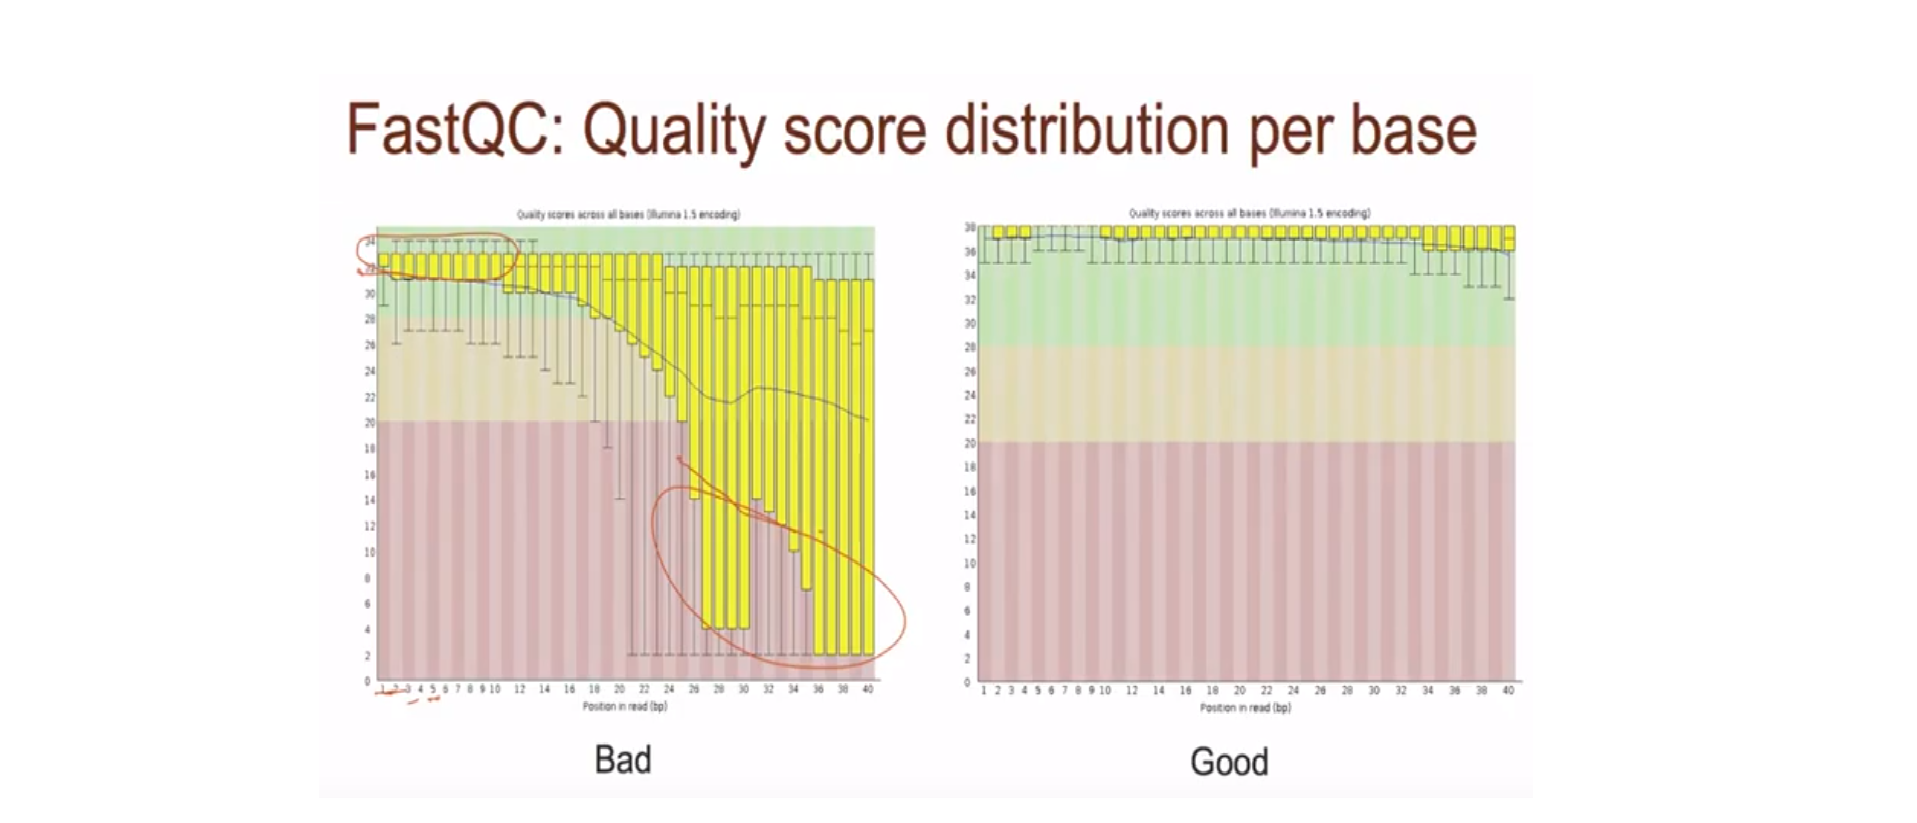
\includegraphics[width=16cm]{Images/Fastqc_Plots1}
  \end{center}
  \caption{Qualité de séquence par base}
  \label{fig-Fastqc_Plots1}
\end{figure}

Cette représentation de la figure 2 nous permet de détecter un sous-ensemble de séquences de basse qualité et de définir un seuil de qualité.

\begin{figure}
  \begin{center}
    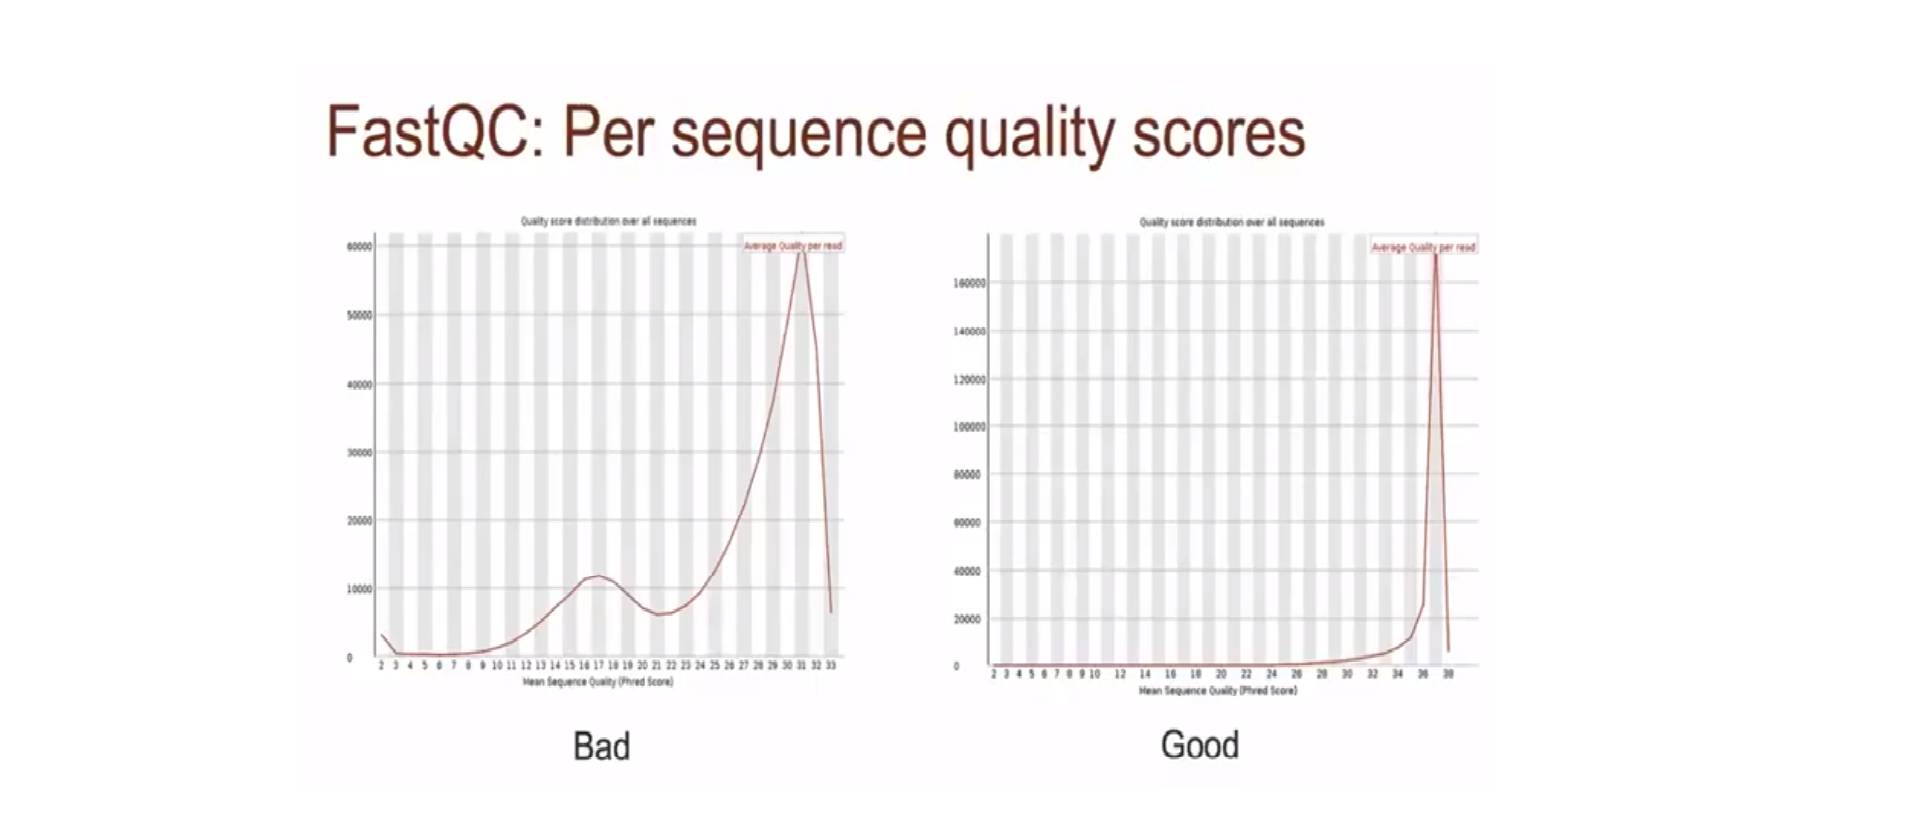
\includegraphics[width=16cm]{Images/Fastqc_Plots2}
  \end{center}
  \caption{Scores de qualité par séquence}
  \label{fig-Fastqc_Plots2}
\end{figure}

La représentation de la figure 3 nous permet de détecter la présence d'adaptateurs ou de mettre en évidence une fragmentation biaisée.

\begin{figure}
  \begin{center}
    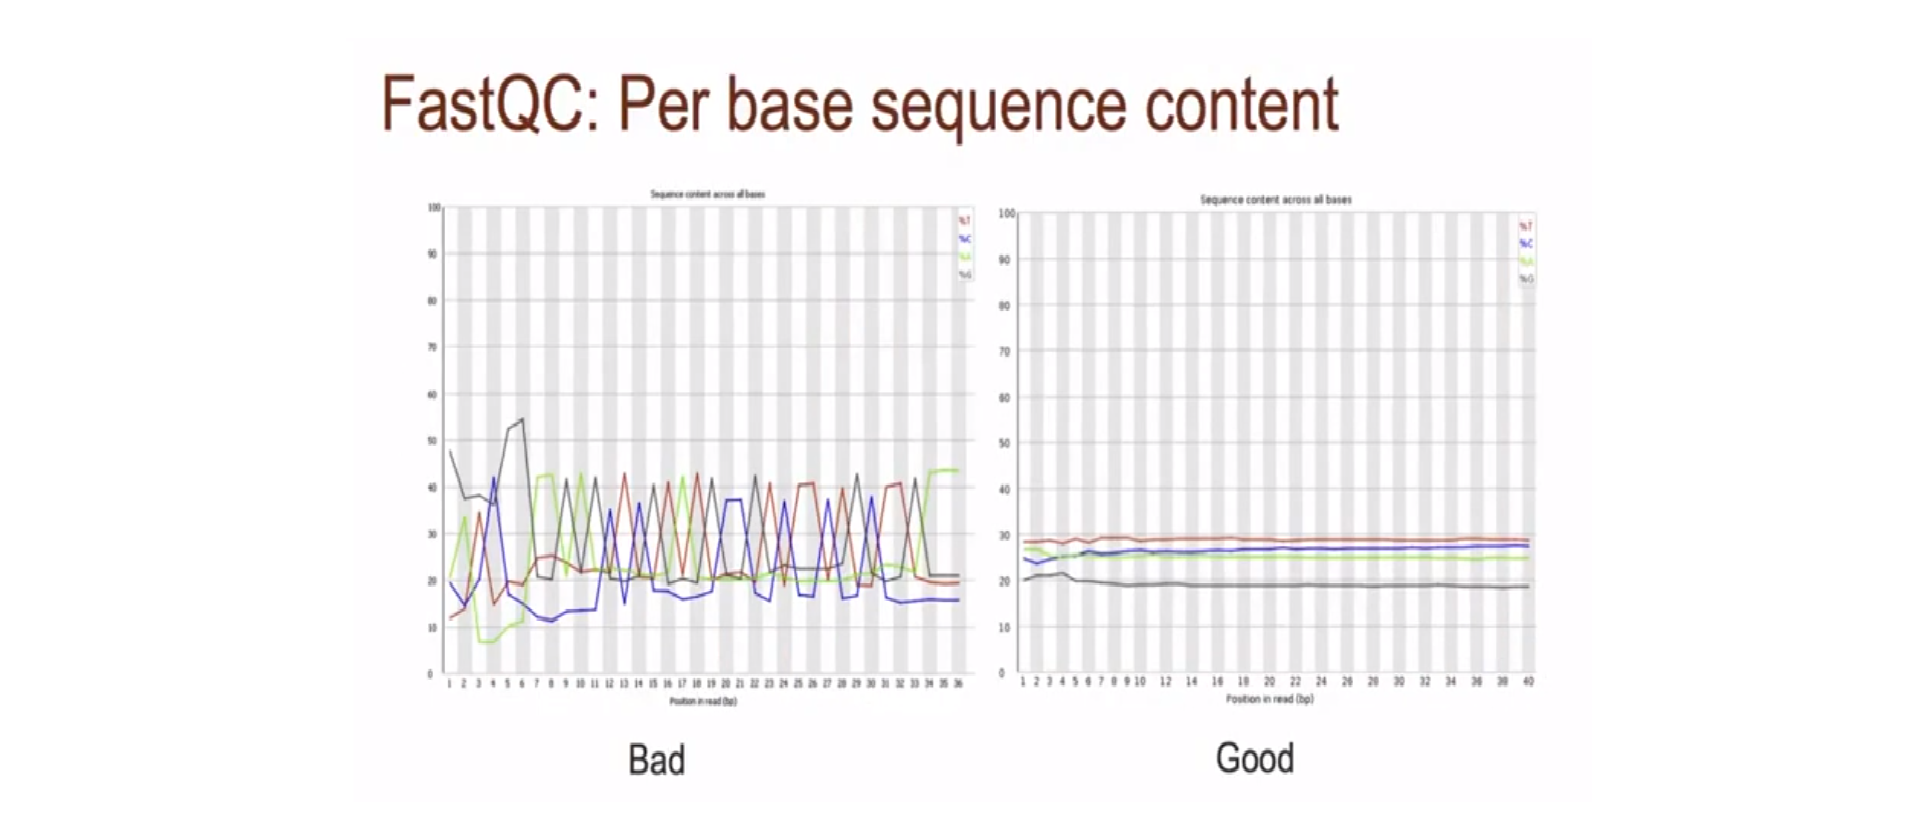
\includegraphics[width=16cm]{Images/Fastqc_Plots3}
  \end{center}
  \caption{Contenu en séquences par base}
  \label{fig-Fastqc_Plots3}
\end{figure}

Dans la figure 4, nous notons des pics en contenu GC, ce qui traduit une éventuelle contamination.

\begin{figure}
  \begin{center}
    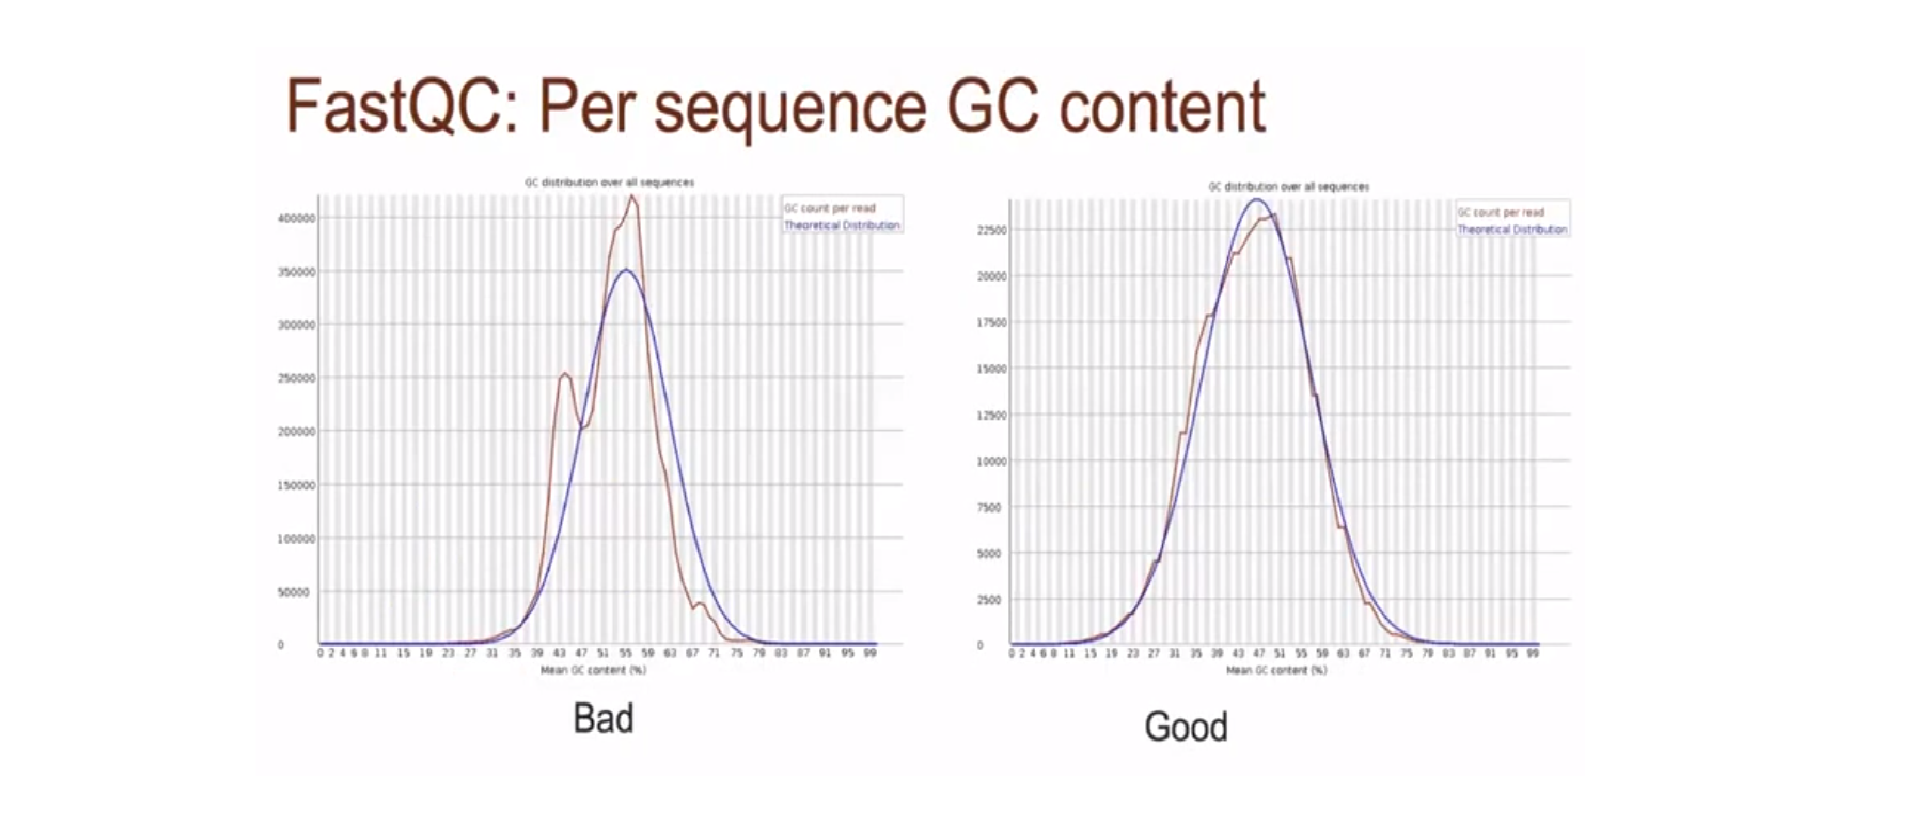
\includegraphics[width=16cm]{Images/Fastqc_Plots4}
  \end{center}
  \caption{Contenu en GC par séquence}
  \label{fig-Fastqc_Plots4}
\end{figure}

Les séquences sur-représentées comme représentées dans la figure 5 sont une indication d'une possible source de contamination.

\begin{figure}
  \begin{center}
    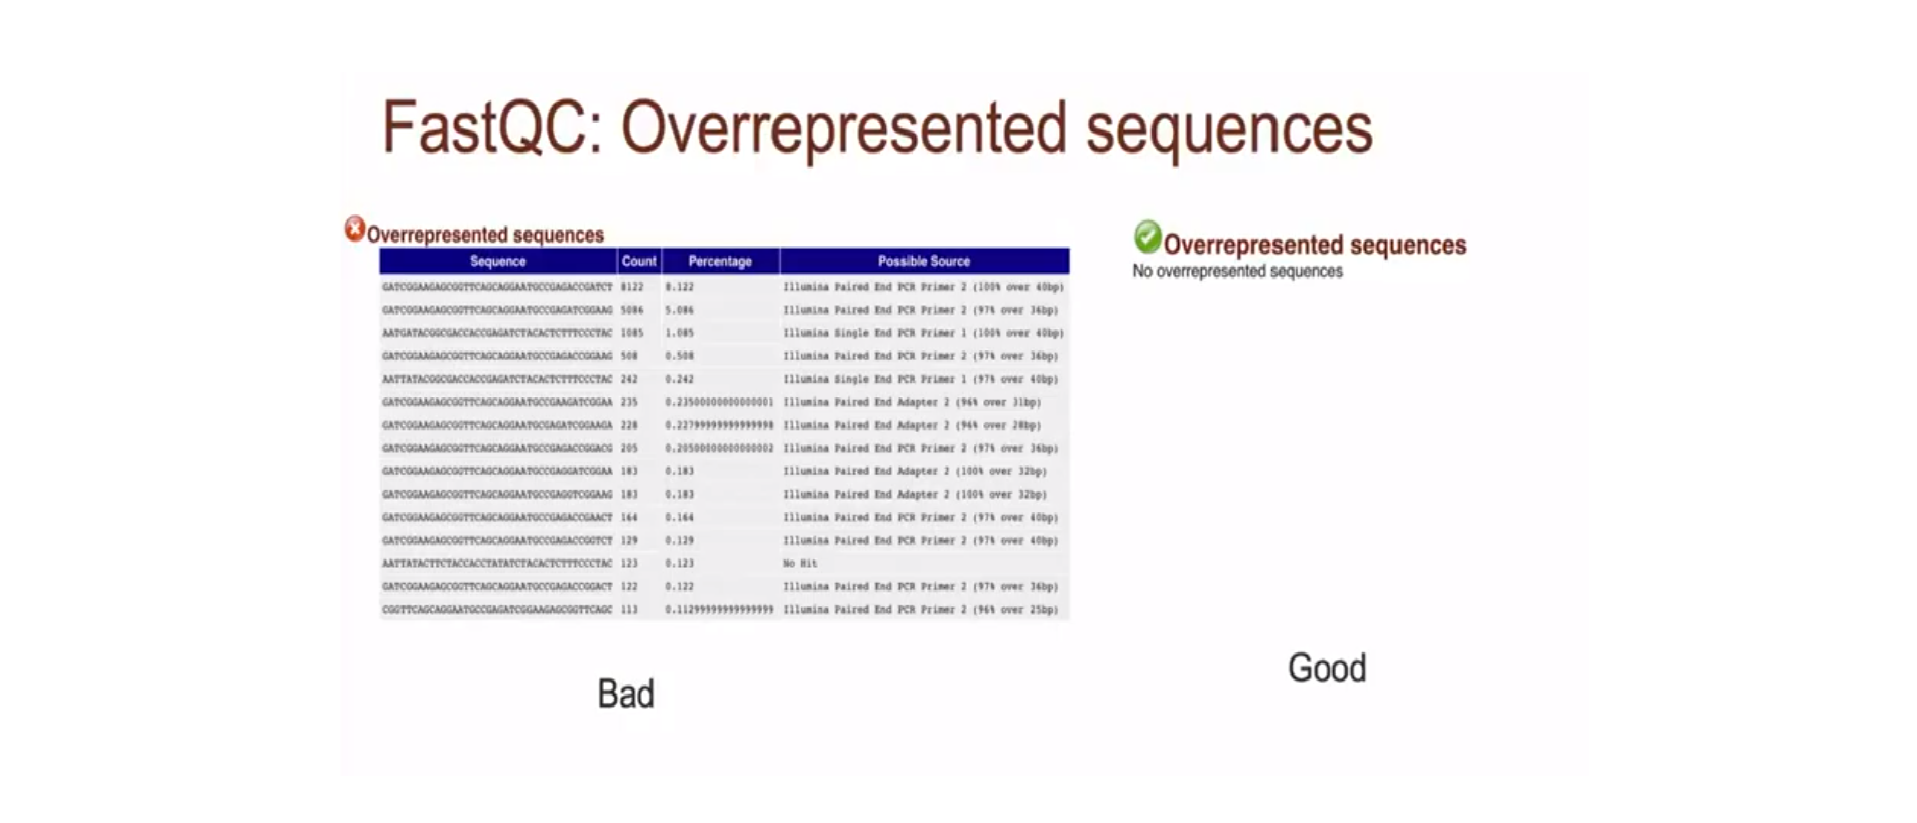
\includegraphics[width=16cm]{Images/Fastqc_Plots5}
  \end{center}
  \caption{Les séquences sur-représentées}
  \label{fig-Fastqc_Plots5}
\end{figure}

La figure 6 nous indique dans le mauvais cas de figure i.e la
représentation de gauche qu'un niveau élevé de duplication est
susceptible d'indiquer un biais d'enrichissement (par exemple, une
suramplification de la PCR).

\begin{figure}
  \begin{center}
    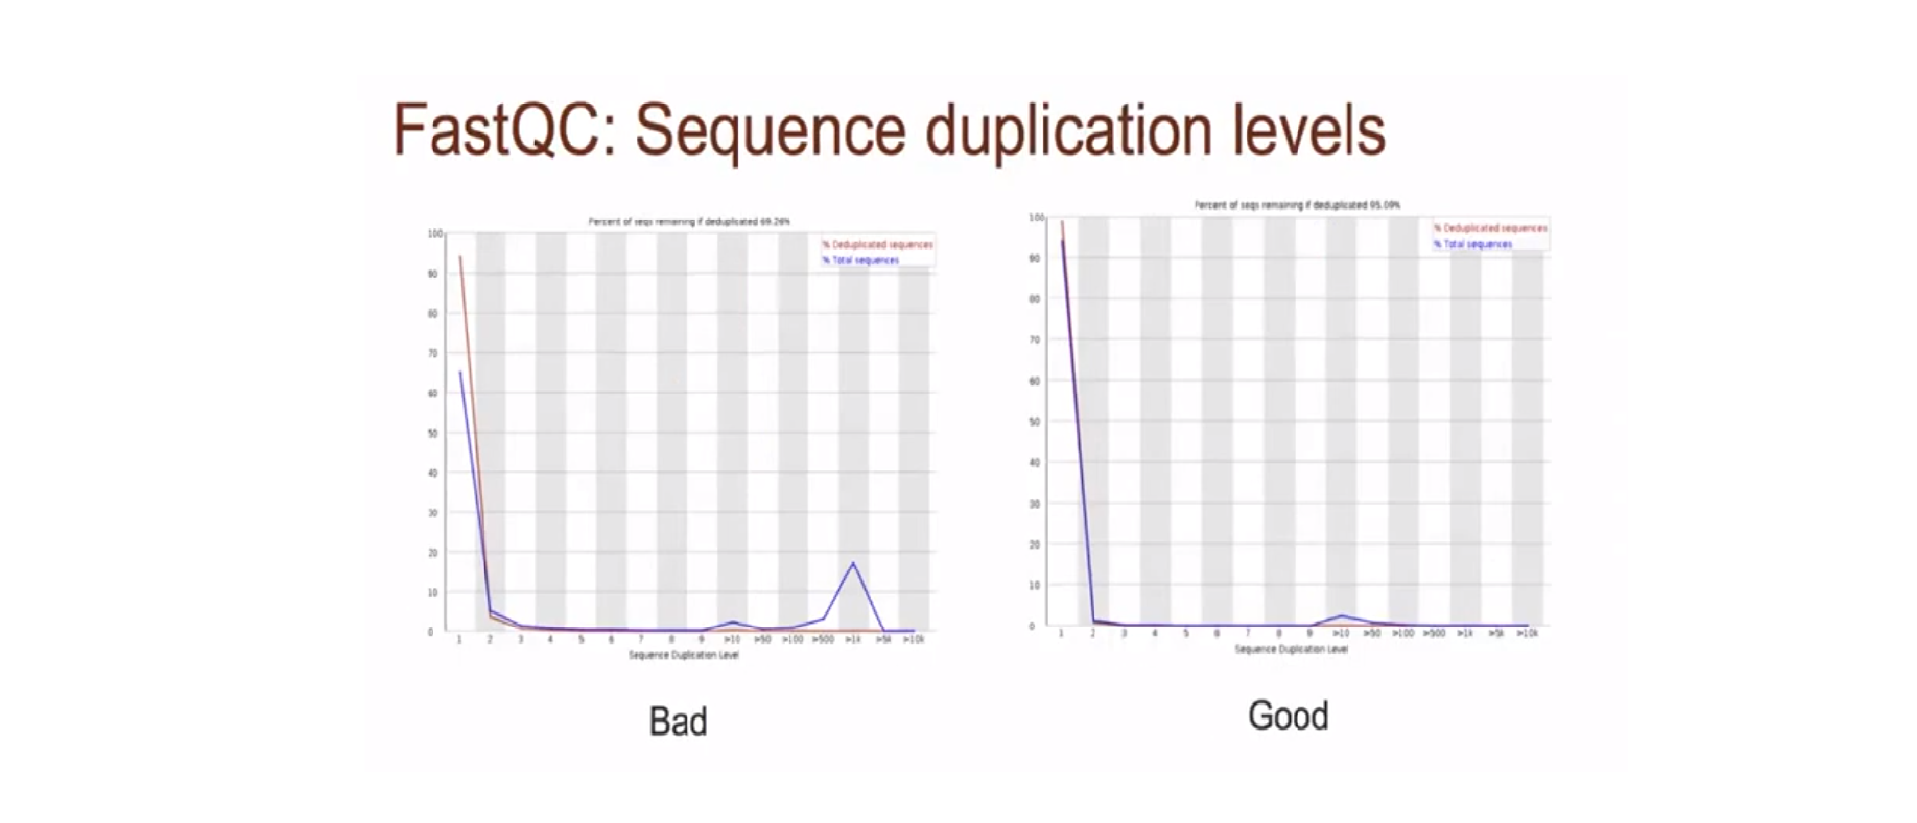
\includegraphics[width=16cm]{Images/Fastqc_Plots6}
  \end{center}
  \caption{Niveaux de duplication par séquence}
  \label{fig-Fastqc_Plots6}
\end{figure}

Sur la figure 7, est illustrée à gauche les problèmes potentiels des cellules d'écoulement (flowcell) d'Illumina.

\begin{figure}
  \begin{center}
    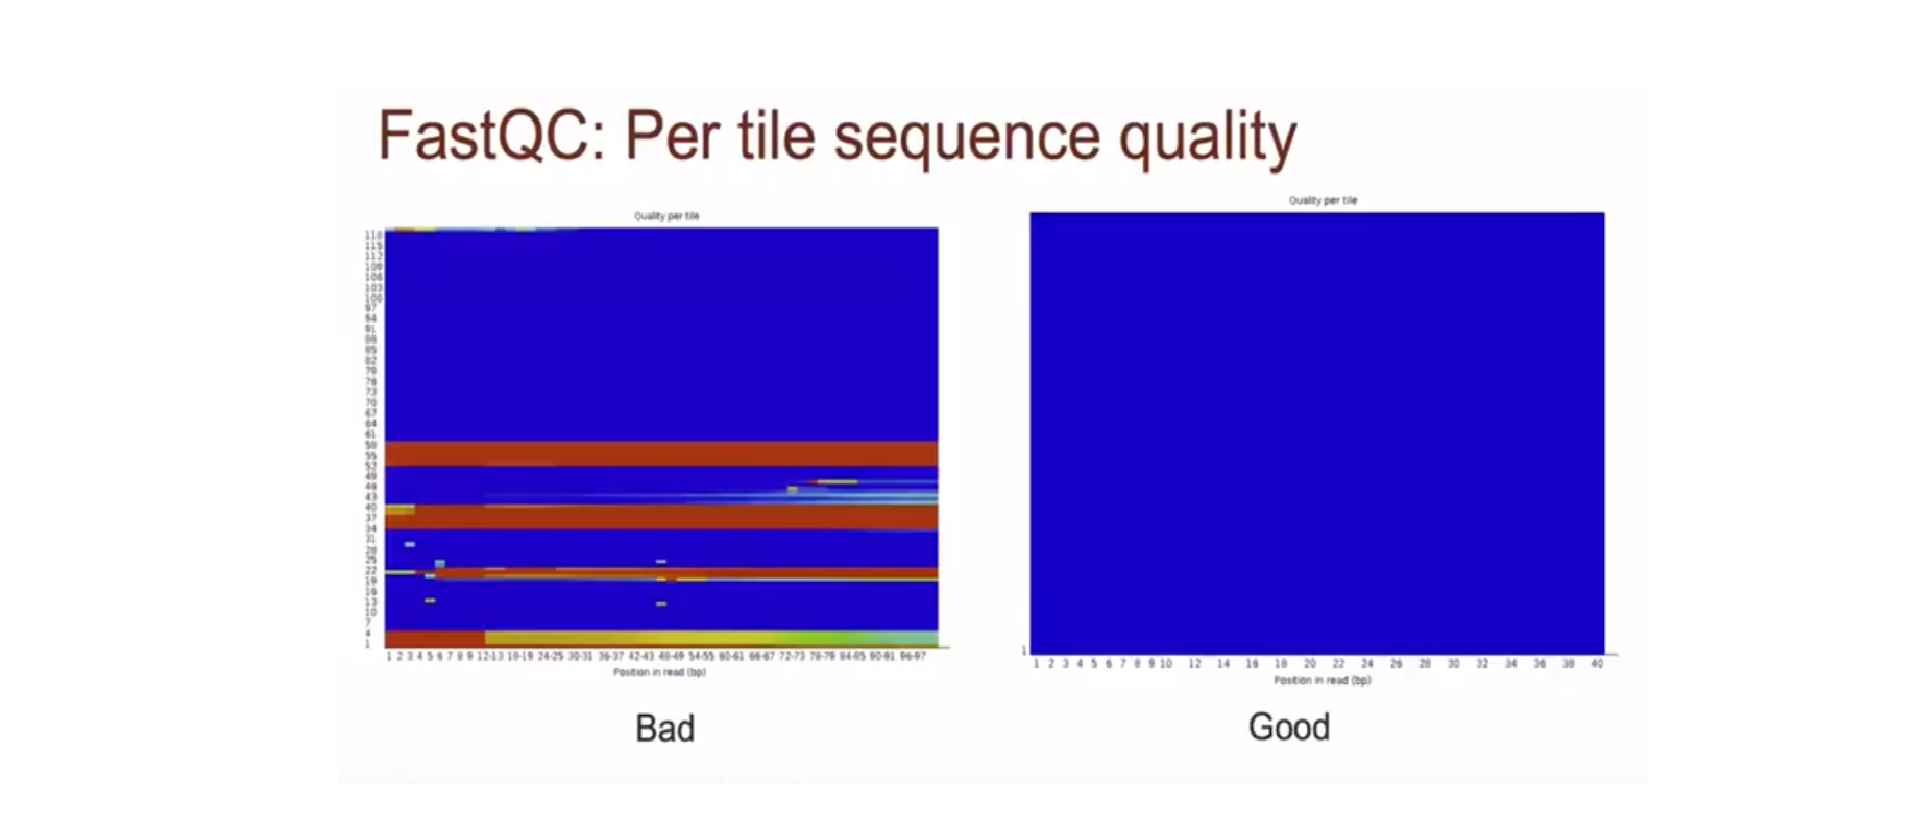
\includegraphics[width=16cm]{Images/Fastqc_Plots7}
  \end{center}
  \caption{Distribution des séquences par taille}
  \label{fig-Fastqc_Plots7}
\end{figure}


\newpage

MultiQC a été développé par Phil
EWELS\footnote{{https://github.com/ewels/MultiQC/tree/master/docs}}. C'est
un outil permettant d’agréger les résultats de la bioinformatique sur
de nombreux échantillons dans un seul rapport. Dans notre cas, nous
utilisons MultiQC pour visualiser les métriques issues de FastQC de tous les
échantillons en un seul rapport(fichier .html).



\end{document}
